% Readout gain at fixed logits (Section "Why the loop can be chaotic"); figure and numbers from
% tools/plot_readout_gain.py (data: ../neural-shrimp-data/explore/llm-soft-loop/readout-gain/p8b).
\begin{figure}[H]
\centering
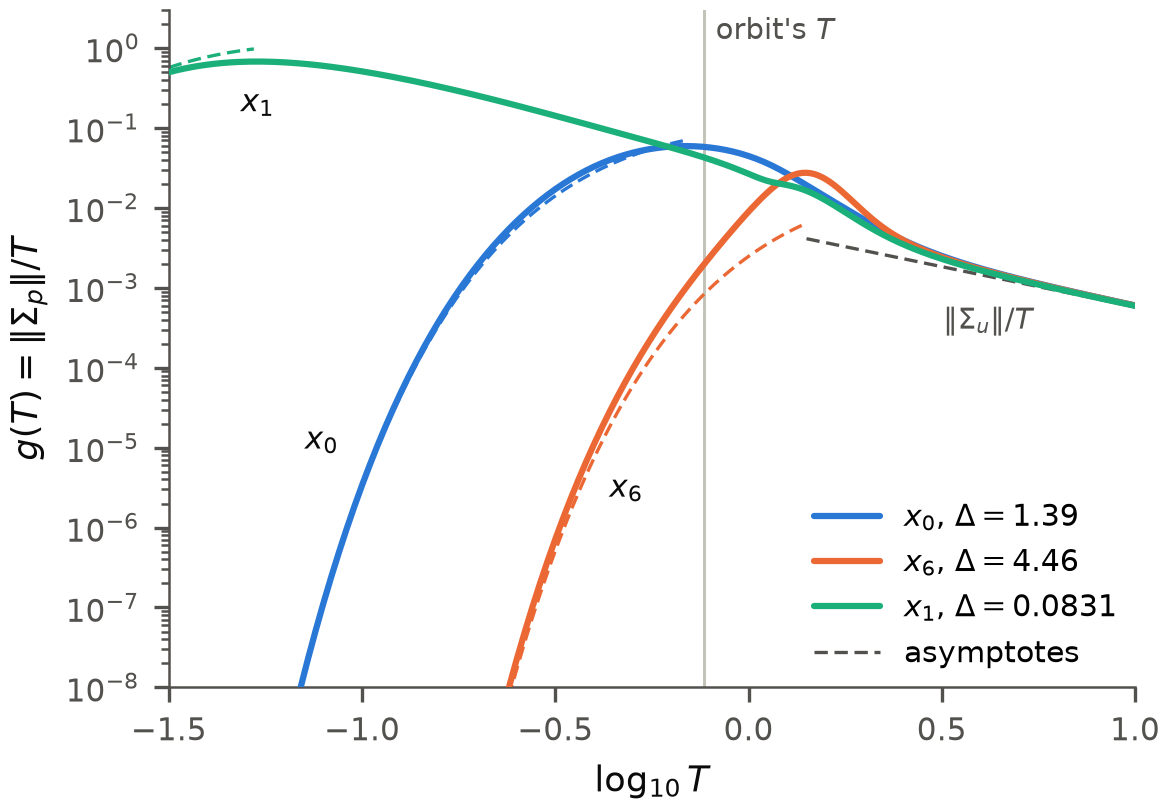
\includegraphics[width=0.6\linewidth]{fig-readout-gain.png}
\caption{Readout gain $g(T)=\|\Sigma_p\|/T$ (spectral norm) at the fixed logits $z_\alpha(x)$ of three states
$x_k=F^k(x_0)$ of the period-8 orbit of Table~\ref{tab:orbits} (Qwen2.5-0.5B-Instruct, philosophy direction at layer
12, $\alpha=0.071674$), with only the temperature in $p=\operatorname{softmax}(z/T)$ varied. $x_0$ is the state at
which \eqref{eq:gain} was checked; $x_6$ and $x_1$ have the largest and the smallest gap $\Delta$ between the two
largest logits among the eight states. Dashed: the low-temperature asymptote $\|e_{t_1}-e_{t_2}\|^2e^{-\Delta/T}/T$ of each
state ($t_1$, $t_2$ the two leading tokens), drawn below its peak, and the high-temperature asymptote $\|\Sigma_u\|/T$,
with $\Sigma_u$ the covariance of all token embeddings under equal weights. The peaks lie at $\log_{10}T=-1.27$ ($x_1$,
$g=0.68$), $-0.16$ ($x_0$, $0.059$) and $0.15$ ($x_6$, $0.028$); the vertical line marks the orbit's temperature,
$\log_{10}T=-0.115$. Where the two leading logits nearly tie ($x_1$), $g$ grows roughly like $1/T$ as $T$ falls toward
$\Delta$. This is the readout factor alone: the network factor $J_{\tilde h}$ is not included, so $g$ does not decide
whether $DF$ expands. At the orbit's temperature $g\le0.064$ at all eight states, while the largest singular value of
$DF$ lies between 1.2 and 21 (Section~\ref{sec:theory}).}
\label{fig:readoutgain}
\end{figure}
